\documentclass[11pt,a4paper]{article}

% Packages
\usepackage[margin=2.5cm]{geometry}
\usepackage{amsmath,amssymb}
\usepackage{graphicx}
\usepackage{booktabs}
\usepackage{hyperref}
\usepackage{listings}
\usepackage{xcolor}
\usepackage{listings}
\usepackage{xcolor}  % For colored syntax highlighting


% Code listing style
\definecolor{codegreen}{rgb}{0,0.6,0}
\definecolor{codegray}{rgb}{0.5,0.5,0.5}
\definecolor{codepurple}{rgb}{0.58,0,0.82}
\definecolor{backcolour}{rgb}{0.95,0.95,0.92}

\lstdefinestyle{mystyle}{
    backgroundcolor=\color{backcolour},   
    commentstyle=\color{codegreen},
    keywordstyle=\color{magenta},
    numberstyle=\tiny\color{codegray},
    stringstyle=\color{codepurple},
    basicstyle=\ttfamily\footnotesize,
    breakatwhitespace=false,         
    breaklines=true,                 
    captionpos=b,                    
    keepspaces=true,                 
    numbers=left,                    
    numbersep=5pt,                  
    showspaces=false,                
    showstringspaces=false,
    showtabs=false,                  
    tabsize=2
}

\lstset{
  language=Python,
  backgroundcolor=\color{backcolour},
  commentstyle=\color{codegreen},
  keywordstyle=\color{magenta},
  numberstyle=\color{codegray},
  stringstyle=\color{codepurple},
  basicstyle=\ttfamily\footnotesize,
  breaklines=true,
  captionpos=b,
  keepspaces=true,
  numbers=left,
  numbersep=5pt,
  showspaces=false,
  showstringspaces=false,
  showtabs=false,
  tabsize=2
}


\lstset{style=mystyle}

\begin{document}

% Custom title page with vertical centering
\begin{titlepage}
    \centering
    \vspace*{\fill}
    
    {\huge\bfseries Reinforcement and Deep Learning\par}
    \vspace{0.5cm}
    {\Large\bfseries Assignment 1\par}
    \vspace{2cm}
    
    {\Large Cadei Paolo\par}
    \vspace{0.5cm}
    {\large Student Number: 14060876\par}
    \vspace{0.5cm}
    {\large Professor: Dr. B.M. (Bram) Wouters\par}
    
    \vspace{2cm}
    
    {\large \today\par}
    
    \vspace*{\fill}
    
\end{titlepage}

\section{Monte Carlo Control for Cliff Walking}

\subsection{Implementation of Monte Carlo Control}
% Your content for 1.a will go here

The Monte Carlo Control algorithm I have implemented in this section is the \textbf{On-policy first-visit MC control (for $\epsilon$-soft policies)} as defined in the book \textbf{Sutton and Barto 2018} (See Section 4.7 for pseudocode).

\begin{lstlisting}
np.random.seed(0)

def has_state_action_pair(states, actions, state, action):
    for i in range(len(states)):
        if states[i] == state and actions[i] == action:
            return True
    return False

# Parameters
epsilon = 0.2       # Epsilon for epsilon-greedy policy
gamma = 0.99        # Discount factor
num_episodes = 10000  # Number of episodes

# Initialize Q-table
Q = np.zeros((cw.nS, cw.nA))  # Q-values initialization
policy = np.ones((cw.nS, cw.nA))/cw.nA #policy initialisation
returns = defaultdict(list)

MC_sum_of_rewards_per_episode = []

for episode in range(num_episodes):

    # Generate an episode using current epsilon-greedy policy
    states, actions, rewards = CW.simulate_episode(cw, Q, epsilon=epsilon, max_iter = 1000)
    
    # Calculate returns for each state-action pair in the episode
    G = 0

    reward = 0
    
    for t in range(len(states) - 2, -1, -1):
        s = states[t]
        a = actions[t]
        r = rewards[t]
        reward += r
        # Calculate return (discounted sum of rewards)
        G = gamma * G + r
        
        # First-visit MC: only update if this is the first occurrence of (s,a)
        if has_state_action_pair(states[:t], actions[:t], s, a):
            continue

        returns[(s, a)].append(G)
        Q[s, a] = np.mean(returns[(s, a)])
        best_actions = np.where(Q[s] == np.max(Q[s]))[0]
        best_action = np.random.choice(best_actions)
             
        policy[s] = epsilon / cw.nA
        policy[s, best_action] = 1 - epsilon + (epsilon / cw.nA)

    MC_sum_of_rewards_per_episode.append(reward)
\end{lstlisting}

\pagebreak

The most important formulas for this algorithm are the following: 
\begin{itemize}
    \item updating function for the action-values using the average of the returns for a specific pair, ensuring convergence to the true value of $Q(S_t, A_t)$: $Q(S_t, A_t) \leftarrow \text{average}(Returns(S_t, A_t))$
    \item $\epsilon$-greedy function which ensures exploration: \(\forall a \in \mathcal{A}(S_t) \):
        \[
        \pi(a|S_t) \leftarrow 
        \begin{cases} 
        1 - \varepsilon + \frac{\varepsilon}{|\mathcal{A}(S_t)|} & \text{if } a = A^* \\ 
        \frac{\varepsilon}{|\mathcal{A}(S_t)|} & \text{if } a \neq A^*
        \end{cases}
        \]
\end{itemize}
\vline

\noindent The idea behind this MC algorithm is that we update the Q-values based on the average returns of only the first occurence of each state-action pair in multiple consecutive episodes. Additionally, the use of an $\epsilon$-greedy policy enables us to balance exploration and exploitation. \\

\noindent It is important to consider the importance of proper initialisation for this algorithm, testified by the variance in running time for the algorithm every run. Setting the appropriate random seed can dramatically impact convergence time, as the first episodes could take a very long time to create due to the stochastic nature of episode generation. It appears that the algorithm's performance is very sensitive to early exploration patterns as well as whole episode creation. If initial states fail to reach terminal states due to poor random walks, convergence can take very long, requiring an excessive number of episodes. \\

\noindent The \textbf{max iter} parameter in the \textbf{simulate episode} function was provided for this reason, however when early episodes consistently not find a terminal state, the algorithm struggles to obtain meaningful return signals, which results in slow and inefficient training. \\

\noindent The four images below show the learning curve of the On-Policy MC Control algorithm as the sum of rewards per episode. They show the difference depending on the random seed used, showing the dependence of the algorithm on the episode creation.

\begin{figure}[h!]
    \centering
    \begin{minipage}{0.55\textwidth}
        \centering
        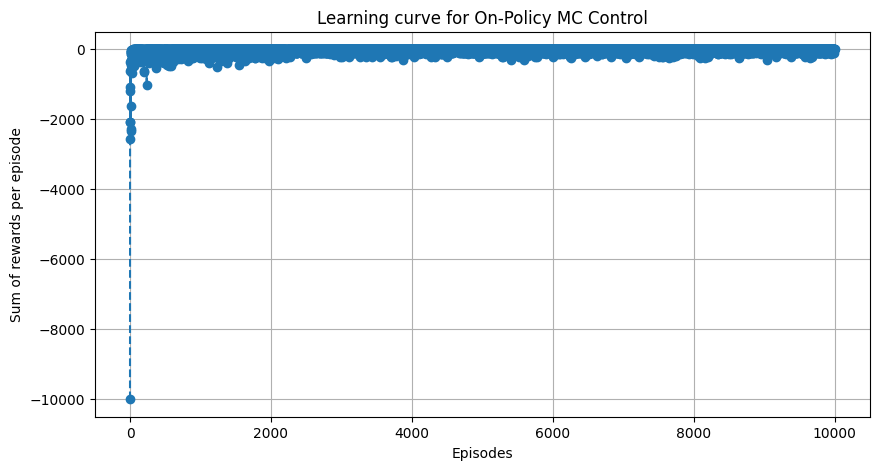
\includegraphics[width=\linewidth]{Assignment1/Images/MC_control_learning_curve.png}
        \caption{Learning curve of On-policy first-visit MC control (for $\epsilon$-soft policies) with random seed = 0}
        \label{fig:fig1}
    \end{minipage}%
    \hfill
    \begin{minipage}{0.4\textwidth}
        \centering
        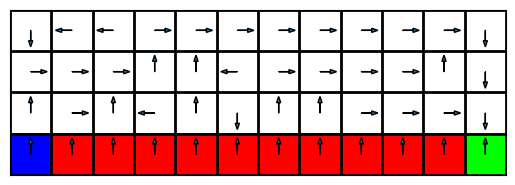
\includegraphics[width=\linewidth]{Assignment1/Images/MC_control_path.png}
        \caption{Path given by implemented On-Policy MC first visit control algorithm with random seed = 0}
        \label{fig:fig2}
    \end{minipage}
\end{figure}

\begin{figure}[h!]
    \centering
    \begin{minipage}{0.55\textwidth}
        \centering
        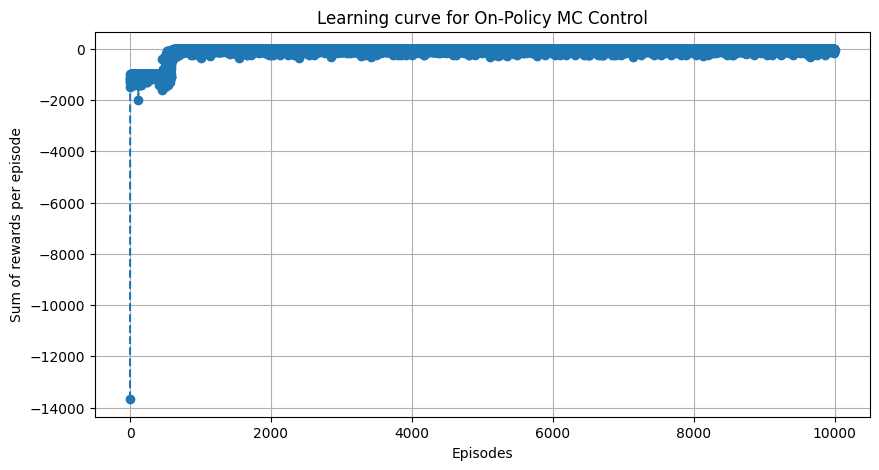
\includegraphics[width=\linewidth]{Assignment1/Images/MC_control_graph2.png}
        \caption{Learning curve of On-policy first-visit MC control (for $\epsilon$-soft policies) without random seed}
        \label{fig:fig1}
    \end{minipage}%
    \hfill
    \begin{minipage}{0.4\textwidth}
        \centering
        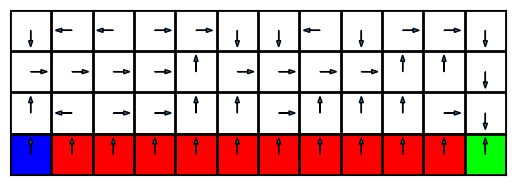
\includegraphics[width=\linewidth]{Assignment1/Images/MC_control_path2.png}
        \caption{Path given by implemented On-Policy MC first visit control algorithm without random seed}
        \label{fig:fig2}
    \end{minipage}
\end{figure}

\pagebreak

\subsection{Comparison with SARSA and Q-LEARNING}

In the following section we will discuss the differences between SARSA, Q-LEARNING and On-Policy MC first visit control algorithms (See Section 4.7 for pseudocode). This discussion will be split into two parts, firstly we will consider the difference between the TD methods SARSA and Q-LEARNING. Then, we will consider the difference between the TD methods and the implemented MC algorithm. Additionally, we will show two different solutions of the implemented MC algorithm which used two different seeds. \\

\noindent The main difference between SARSA and Q-LEARNING is that, while both are TD methods, they are on-policy and off-policy respectively. This is shown in how they estimate future returns: SARSA uses $a_{t+1}, s_{t+1}$, taking into account the exploration policy it follows, while Q-LEARNING uses the maximum possible Q-value from the next state, without considering which action might actually be taken by the policy. This is shown by the following formulas:
\begin{itemize}
    \item SARSA: $Q(S, A) \leftarrow Q(S, A) + \alpha \left[ R + \gamma Q(S', A') - Q(S, A) \right]$ where $A'$ and$ S'$ are chosen using the policy derived from $Q$.
    \item Q-LEARNING: $Q(S, A) \leftarrow Q(S, A) + \alpha \left[ R + \gamma \max_a Q(S', a) - Q(S, A) \right]$

\end{itemize}

\begin{figure}[h!]
    \centering
    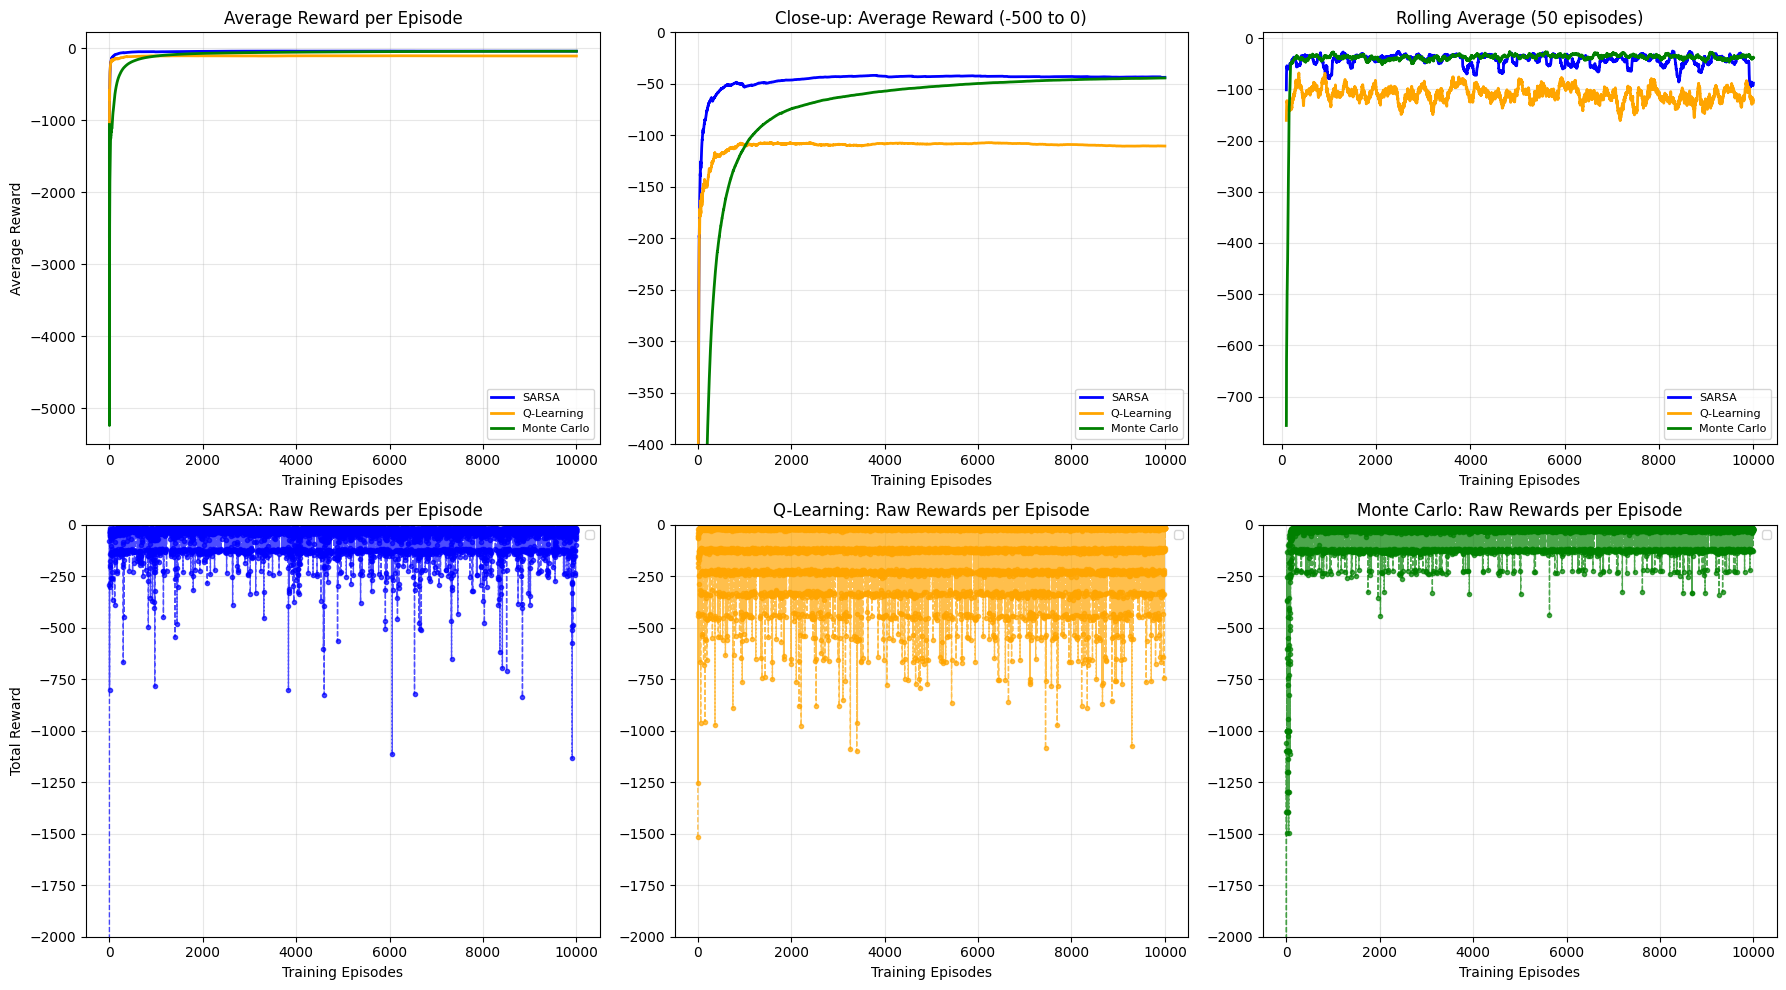
\includegraphics[width=0.8\textwidth]{Assignment1/Images/MC_Sarsa_Q.png}
    \caption{Graphs of different metrics for the learning curves of SARSA, Q-LEARNING and implemented MC Control}
\end{figure}

The difference in these methods makes \textbf{SARSA more conservative}, prioritising "safety" during exploration, and \textbf{Q-LEARNING more risky}. All in all, SARSA learns the safer path further from the cliff while Q-LEARNING, focusing on optimal paths, learns the shorter route which is lastly the optimal one but that suffers during training as it falls more often in the cliff (See Section 4.1 in the Appendix). The former observations align with what is shown in Figure 5: both SARSA and Q-LEARNING show an immediate improvement in the policy (See top-left graph) with a big increase in rewards per episode. However, after this big jump, Q-LEARNING stabilises at a lower average reward compared to SARSA (See top-center graph). \\

\noindent Now, we will be discussing the difference between the two TD methods and the implemented MC Control algorithm. The main difference between these methods is that the former algorithms update estimates at each step while \textbf{MC methods wait until the end of a complete episode before updating values}. This main difference means that MC methods will initially show poor performance and will take longer than the other two methods to get better (See top-center and top-left graphs above and for even bigger difference See Section 4.2 in the Appendix). MC eventually improves, approaching SARSA's performance level (See top-center graph). \\


\noindent The former observations are mainly due to the nature of the algorithms. However, this nature also affects the amount of time the algorithm takes to train. While SARSA and Q-LEARNING are relatively fast and converge to the same solution with a very similar amount of time for each iteration, MC algorithms take a lot longer and they are also sensitive to initialisation conditions, leading to high variance in the amount of time and episodes taken for training (See Section 1.1).\\

\noindent All in all, SARSA and the MC Control policy ($\epsilon = 0.2$), both being on-policy methods, ultimately learn similar conservative policies, prioritising safety during exploration and therefore converging to higher average rewards then Q-LEARNING. Q-LEARNING, as an off-policy, learns a riskier policy that performs worse if the average rewards during training are considered. 

\section{Taxi Environment Analysis}

The following function is used in the implementation of both SARSA and Q-LEARNING: \\

\begin{lstlisting}
def select_action(state, Q, action_mask, epsilon=0.0):

    # Extract indices of allowed actions
    valid_actions = np.where(action_mask == 1)[0]
    if np.random.rand() < epsilon:
        action_ = np.random.choice(valid_actions)
    else:
        q_values_valid = Q[state][valid_actions]
        max_q = np.max(q_values_valid)
        # In case multiple actions have the same max Q-value, randomly choose among them
        best_actions = valid_actions[q_values_valid == max_q]
        action_ = np.random.choice(best_actions)

    return action_
\end{lstlisting}

\vline

\noindent In the following implementations it is also important to note that I have used the allowed actions provided by the environment for each state, which leads to faster convergence and less computational time. For the code that doesn't use the allowed actions please check the Appendix (See Section 4.3, 4.4 and 4.5).

\subsection{SARSA Implementation}

The following code shows my implementation of the SARSA algorithm for the Taxi environment implemented in Gymnasium: \\

\begin{lstlisting}
alpha = 0.1
gamma = 0.99
num_episodes = 10000
epsilon = 0.1
Q = np.zeros((env.observation_space.n, env.action_space.n))
sarsa_sum_of_rewards_per_episode = []

for episode in range(num_episodes):

    rewards = []
    # random state and i['action_mask] contains the actions that can be taken
    s, i = env.reset()
    a = select_action(s, Q, i['action_mask'], epsilon)

    while True:

        s_prime, r, is_done, is_terminated, i_prime = env.step(a)
        a_prime = select_action(s_prime, Q, i_prime['action_mask'], epsilon)
        
        Q[s, a] += alpha * (r + gamma * Q[s_prime, a_prime] - Q[s, a])

        s = s_prime
        a = a_prime
        rewards.append(r)

        if is_done or is_terminated:
            break
    
    sarsa_sum_of_rewards_per_episode.append(np.sum(rewards))
\end{lstlisting}

\subsection{Q-LEARNING Implementation}

The following code shows my implementation of the Q-LEARNING algorithm for the Taxi environment implemented in Gymnasium: \\

\begin{lstlisting}
alpha = 0.1
gamma = 0.99
epsilon = 0.1
num_episodes = 10000

Q = np.zeros((env.observation_space.n, env.action_space.n))

q_sum_of_rewards_per_episode = []

for episode in range(num_episodes):

    '''if (episode + 1) % 10000 == 0:
        print(f"Episode {episode + 1}/{num_episodes}")'''

    rewards = []
    # random state and i['action_mask] contains the actions that can be taken
    s, i = env.reset()

    while True:
    
        a = select_action(s, Q, i['action_mask'], epsilon)
        s_prime, r, is_done, is_terminated, i_prime = env.step(a)
        rewards.append(r)

        mask = i_prime['action_mask']
        valid_actions = np.where(mask == 1)[0]
        q_values_valid = Q[s_prime][valid_actions]
        max_q = np.max(q_values_valid)

        Q[s, a] += alpha * (r + gamma * max_q - Q[s, a])

        if is_done or is_terminated:
            break

        s = s_prime
        i = i_prime
    
    q_sum_of_rewards_per_episode.append(np.sum(rewards))
\end{lstlisting}



\subsection{Performance Comparison}

% First paragraph with image and text
\noindent
\begin{minipage}{0.5\textwidth}
    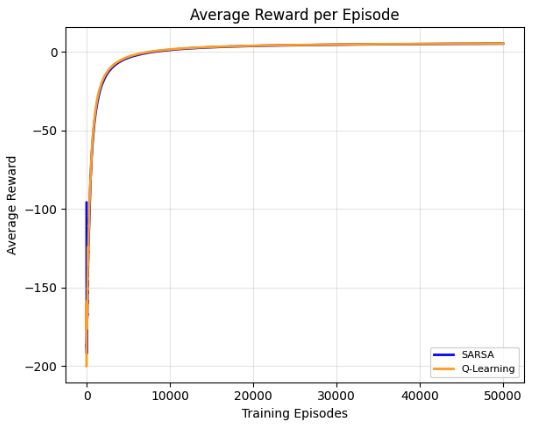
\includegraphics[width=\linewidth]{Assignment1/Images/Taxi_sarsa_q1.png}
\end{minipage}%
\hfill%
\begin{minipage}{0.45\textwidth}
    The graph on the left shows that there is a minimal difference between the two methods for the Taxi driver. However, there are a couple things that we should consider and to do this we will be zooming in on the graph: firstly, we will consider the initial episodes, and then we will take a look at the graph when the average episode rewards have already increased.
\end{minipage}

% Second paragraph with image and text
\noindent
\begin{minipage}{0.5\textwidth}
    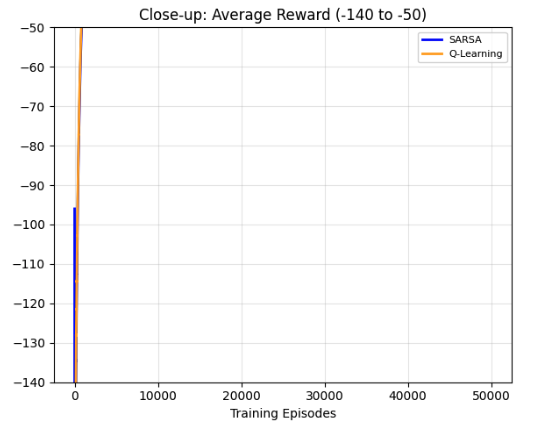
\includegraphics[width=\linewidth]{Assignment1/Images/Taxi_sarsa_q2.png}
\end{minipage}%
\hfill%
\begin{minipage}{0.45\textwidth}
    Zooming in on the \textbf{initial training episodes}, we can see that SARSA performs slightly better at the beginning than Q-LEARNING (considering it is a very small difference). This is due to the nature of the algorithms: SARSA follows a more conservative approach, prioritising immediate performance during learning rather than optimising for an eventual perfect policy. This means that SARSA initially outperforms Q-LEARNING because it accounts for exploration risk, creating a "safer" policy during early training when random actions are frequent.
\end{minipage}

% Third paragraph with image and text
\noindent
\begin{minipage}{0.5\textwidth}
    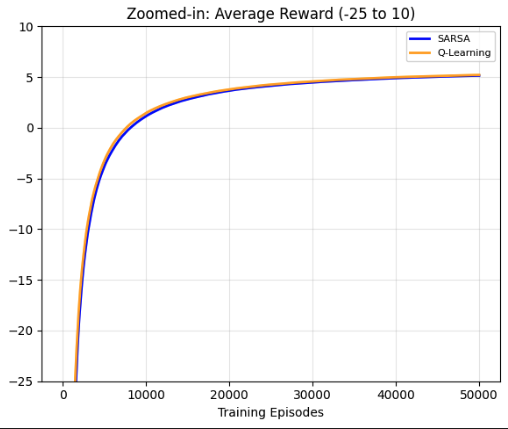
\includegraphics[width=\linewidth]{Assignment1/Images/Taxi_sarsa_q3.png}
\end{minipage}%
\hfill%
\begin{minipage}{0.45\textwidth}
    Zooming in for the \textbf{episodes with higher average episode rewards}, we can see that Q-LEARNING leads to better final performance. This is due to the fact that Q-LEARNING optimises directly the optimal greedy policy which results in higher performance once exploration dimishes since the Q-LEARNING's updates are already aligned with the optimal policy when exploration decreases.
\end{minipage}

\vline

It is interesting to note the difference between the Cliff-Walking and the Taxi environments for Q-LEARNING and SARSA performances. In the former, SARSA achieves better results while in the latter, Q-LEARNING has a better performance. This is also due to the safer environment in Taxi Driver as there are no "catastrophic" failures as there are in Cliff-Walking, making Q-LEARNING less "risky".

\section{Additional Analysis}

For the additionaly analysis I will be considering multiple "frameworks": firstly, I will check the \textbf{influence of $\alpha$ on the TD methods}, then I will check the\textbf{ influence of epsilon} on both the TD methods and the implemented MC control algorithm, and finally, I will implement the MC control method with \textbf{$\epsilon$-decay}.

\subsection{$\alpha$ analysis}

The following analysis was conducted by simply running the algorithms (See Sections 2.1 and 2.2) on multiple values of $\alpha$ and then storing their rewards for visualisation.

\begin{figure}[h!]
    \centering
    \begin{minipage}{0.47\textwidth}
        \centering
        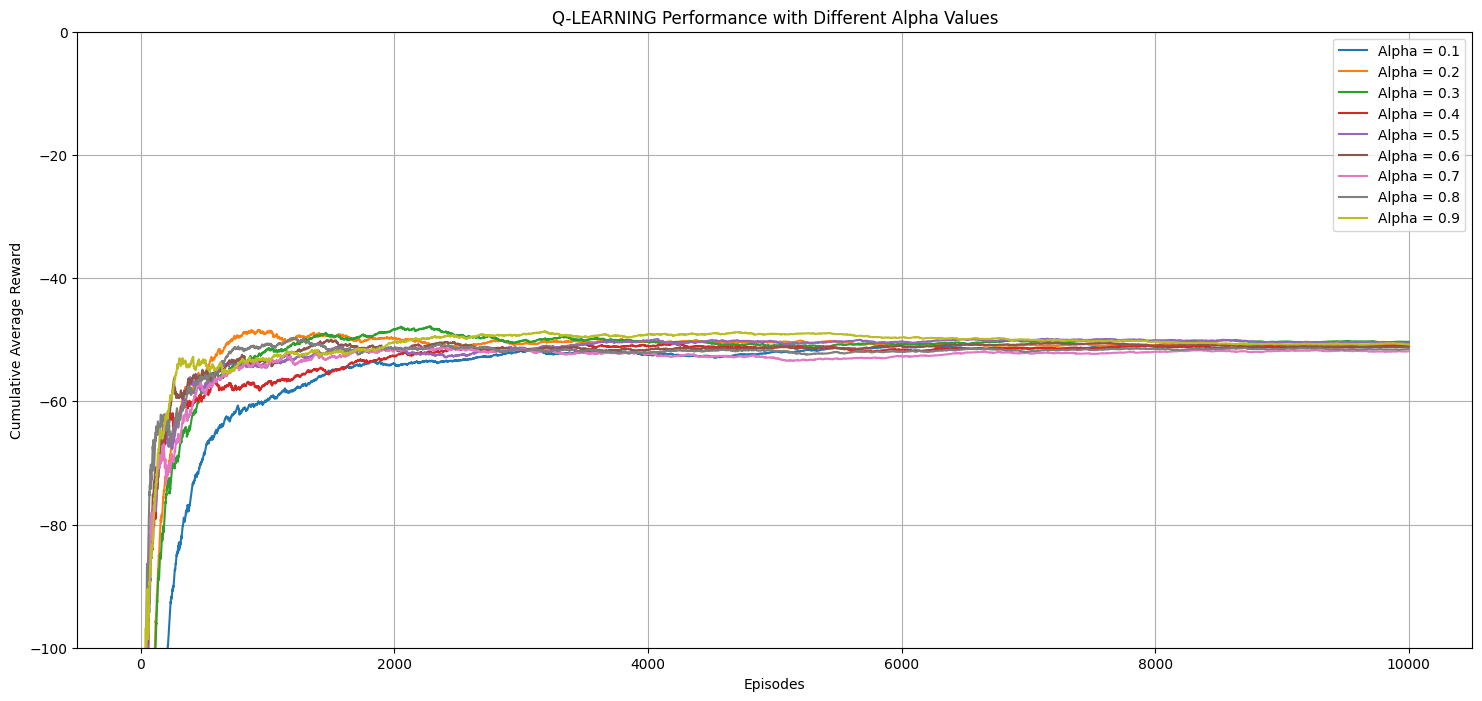
\includegraphics[width=\linewidth]{Assignment1/Images/alpha_q.png}
        \caption{Learning curve for different $\alpha$ values for Q-LEARNING}
        \label{fig:fig1}
    \end{minipage}%
    \hfill
    \begin{minipage}{0.47\textwidth}
        \centering
        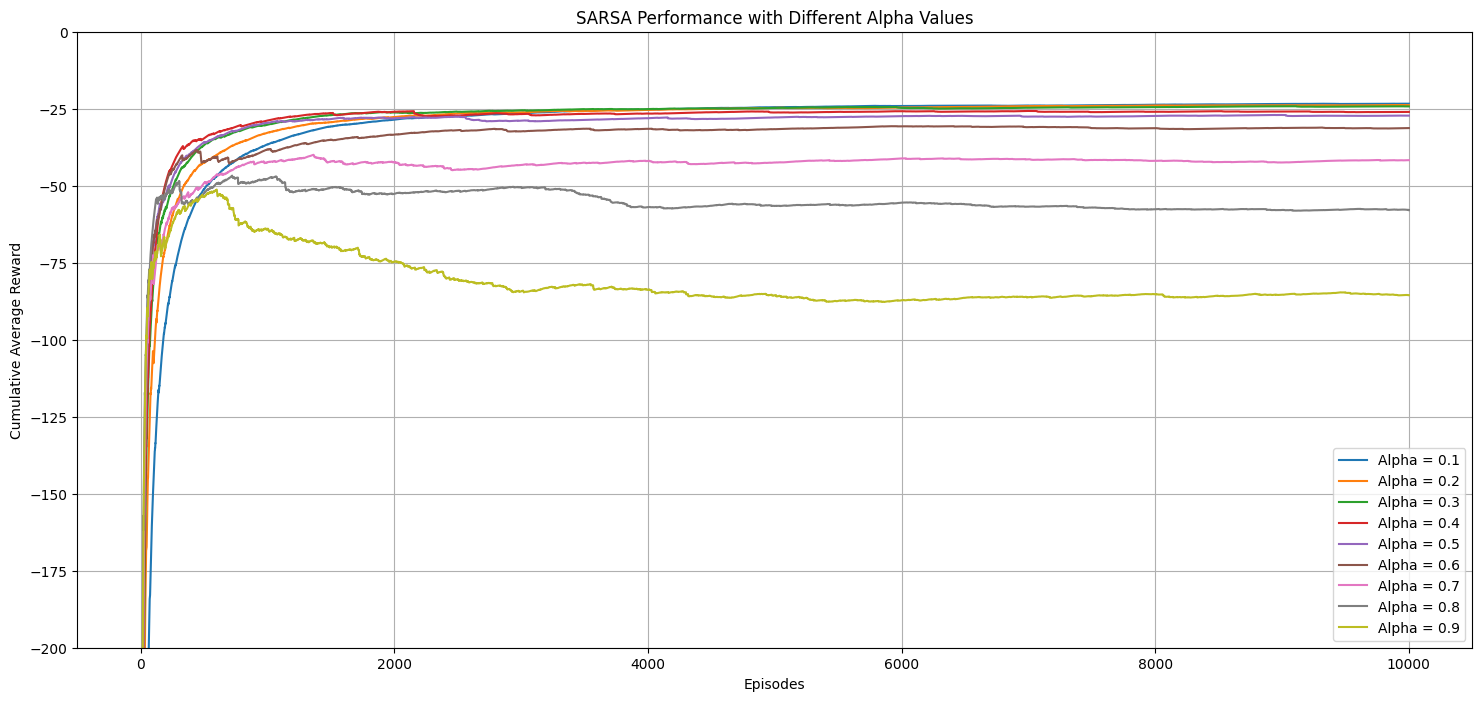
\includegraphics[width=\linewidth]{Assignment1/Images/alpha_sarsa.png}
        \caption{Learning curve for different $\alpha$ values for SARSA}
        \label{fig:fig2}
    \end{minipage}
\end{figure}

\vline

The images above show how changing the \textbf{learning rate parameter ($\alpha$)} affects the performance and convergence of Q-LEARNING and SARSA in the Cliff-Walking environment.\\

For \textbf{Q-LEARNING}, we can see that higher learning rates lead to a steeper learning curve, meaning that they enable the model to achieve a good performance level with fewer episodes. On the other hand, for lower learning rates, convergence takes more time but the performance increases in a more stable way than with higher values. Additionally, the algorithms achieve stable performance with all different learning rates tested, leading to a similar average reward. \\

For \textbf{SARSA}, we can see that higher learning rates lead to a steeper increase than lower ones. However, this increase is not sustained as the higher learning rates' rewards tend to drop sharply right after the initial increase. Additionally, the average rewards experience a significant decrease after many episodes for higher $\alpha$ values. On the other hand, lower $\alpha$
values create safer paths which increase rewards in a slower but steadier way (less major "regressions"). \\

Overall, \textbf{Q-LEARNING's convergence is more robust to a change in learning rate} as the algorithm doesn't suffer even with learning rates approaching $1.0$. Conversely, SARSA is more sensitive to changes in $\alpha$.

\vline

\subsection{$\epsilon$ analysis}

I have run the code for this analysis and the images can be found in the Appendix (See Section 4.6 in the Appendix). However, only the images are going to be provided in this case.

\vline

\subsection{$\epsilon$-decay}

In the following section we will be applying $\epsilon$-decay to the algorithm we previous implemented, namely On-policy first-
visit MC control (for $\epsilon$-soft policies). The idea behind $\epsilon$-decay is initialising epsilon to a very high value and then gradually decreasing it by a specified decay-rate until it reaches a defined minimum value. The pseudocode for this would be:

\begin{lstlisting}
    epsilon = 1 # this is the initial value of epsilon
    epsilon_decay_rate = 0.9995
    epsilon_minimum = 0.2 # mimum value that epsilon can take

    Loop through the episodes
        ...

    epsilon <- max(epsilon_minimum, epsilon * epsilon_decay_rate)
\end{lstlisting}

\vline

Additionally, we will compare the initial results to the ones given by the new implemenation. \\

\begin{lstlisting}
def has_state_action_pair(states, actions, state, action):
    for i in range(len(states)):
        if states[i] == state and actions[i] == action:
            return True
    return False

# Parameters
epsilon = 1      # Epsilon for epsilon-greedy policy
gamma = 0.99        # Discount factor
num_episodes = 10000  # Number of episodes
epsilon_decay_rate = 0.9995 # Decay rate per episode
min_epsilon = 0.1

Q = np.zeros((cw.nS, cw.nA))  # Q-values initialization
policy = np.ones((cw.nS, cw.nA))/cw.nA #policy initialisation
returns = defaultdict(list)
MC_sum_of_rewards_per_episode = []

for episode in tqdm(range(num_episodes), desc="Training Episodes"):
    # Generate an episode using current epsilon-greedy policy
    states, actions, rewards = CW.simulate_episode(cw, Q, epsilon=epsilon, max_iter=1000)
    
    # Calculate returns for each state-action pair in the episode
    G = 0
    reward = 0
    
    for t in range(len(states) - 2, -1, -1):
        s = states[t]
        a = actions[t]
        r = rewards[t]

        reward += r
        
        # Calculate return (discounted sum of rewards)
        G = gamma * G + r
        
        # First-visit MC: only update if this is the first occurrence of (s,a)
        if has_state_action_pair(states[:t], actions[:t], s, a):
            continue

        returns[(s, a)].append(G)
        Q[s, a] = np.mean(returns[(s, a)])

        best_actions = np.where(Q[s] == np.max(Q[s]))[0]
        best_action = np.random.choice(best_actions)
             
        policy[s] = epsilon / cw.nA
        policy[s, best_action] = 1 - epsilon + (epsilon / cw.nA)

    MC_sum_of_rewards_per_episode.append(reward)

    # Decay epsilon
    epsilon = max(min_epsilon, epsilon * epsilon_decay_rate)
\end{lstlisting}

\begin{figure}[h!]
    \centering
    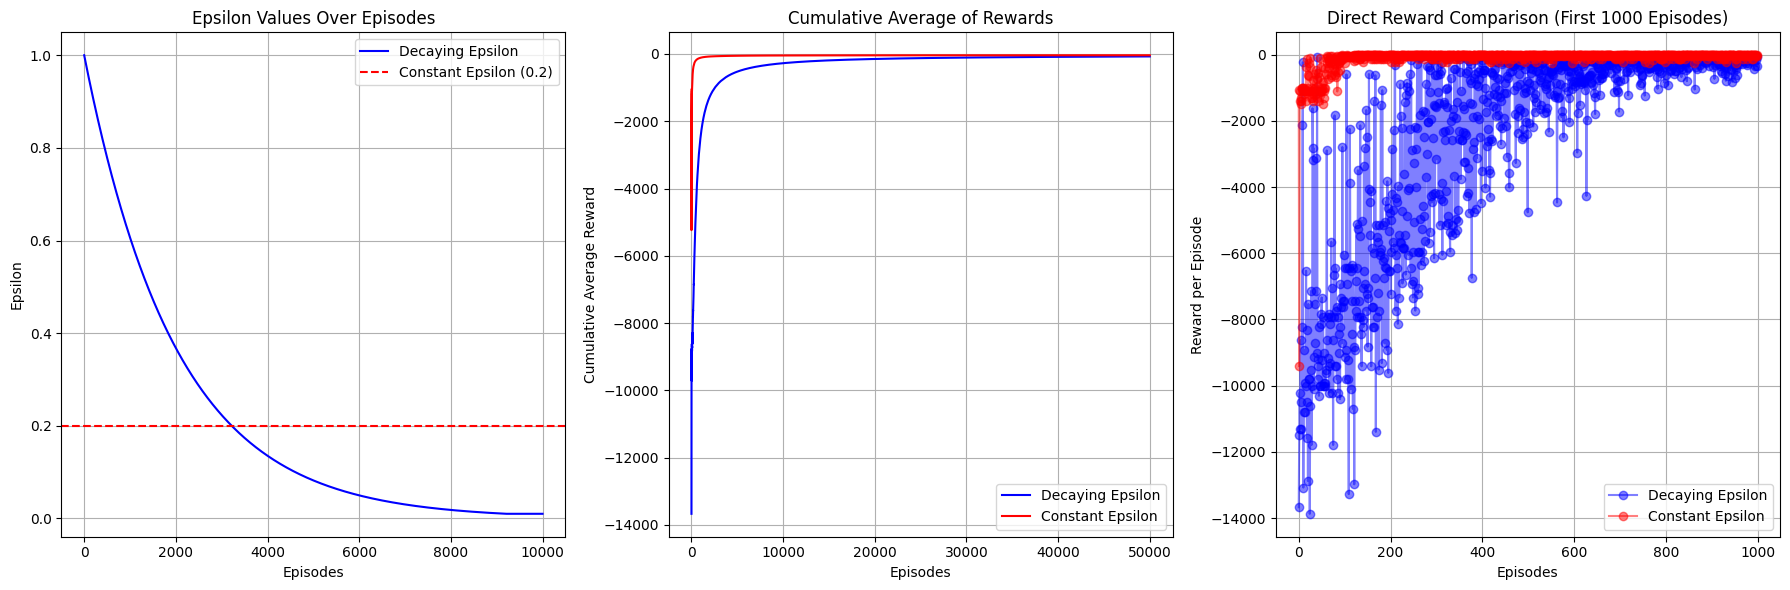
\includegraphics[width=1\textwidth]{Assignment1/Images/mc_vs_edecay.png}
    \caption{Performance comparison between MC with constant $\epsilon$ and $\epsilon$-decay}
    \label{fig:yourlabel}
\end{figure}

From the graphs provided we see the following:
\begin{itemize}
    \item \textbf{1st graph (left)}: shows the decrease in $\epsilon$ which means that the agent explores more in the early stages and exploits more towards the end of training. The constant epsilon, on the other hand, mantains a balance between exploration and exploitation
    \item \textbf{2nd graph (center)}: shows that the constant $\epsilon$ leads to faster initial learning while decaying $\epsilon$ takes longer to converge as it prioritises exploration early on. Ultimately, both algorithms converge to similar average rewards.
    \item \textbf{3rd graph (right)}: shows the high variability in early episodes of the model with $\epsilon$-decay due to the extensive exploration, as compared to the lower variance of the algorithm with $\epsilon$ kept constant.
\end{itemize}

Overall, while the constant epsilon algorithm achieves faster initial learning, decaying epsilon is more robust for the long-term optimisation as it reduces exploration once information about the environment has been acquired. The difference in performance that $\epsilon$-decay can achieve is not portrayed here as the environment is quite simple and very little exploration is needed in this case.

\pagebreak


\section{Appendix}

\subsection{SARSA and Q-LEARNING paths}

\begin{figure}[h!]
    \centering
    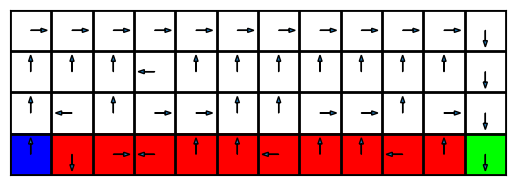
\includegraphics[width=0.5\textwidth]{Assignment1/Images/path_sarsa.png}
    \caption{SARSA's path}
    \label{fig:yourlabel}
\end{figure}

\begin{figure}[h!]
    \centering
    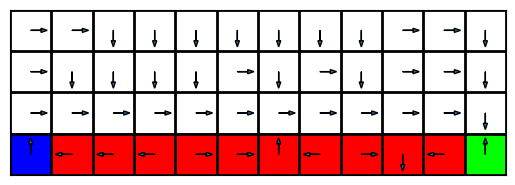
\includegraphics[width=0.5\textwidth]{Assignment1/Images/path_q.png}
    \caption{Q-LEARNING's path}
    \label{fig:yourlabel}
\end{figure}

\begin{figure}[h!]
    \centering
    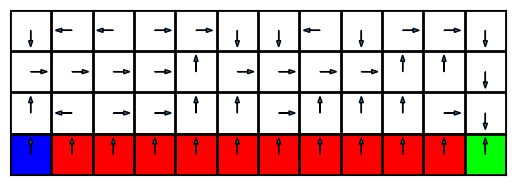
\includegraphics[width=0.5\textwidth]{Assignment1/Images/path_mc.png}
    \caption{MC's path}
    \label{fig:yourlabel}
\end{figure}

\subsection{Graphs comparing SARSA, Q-Learning, and implemented MC.}

\begin{figure}[h!]
    \centering
    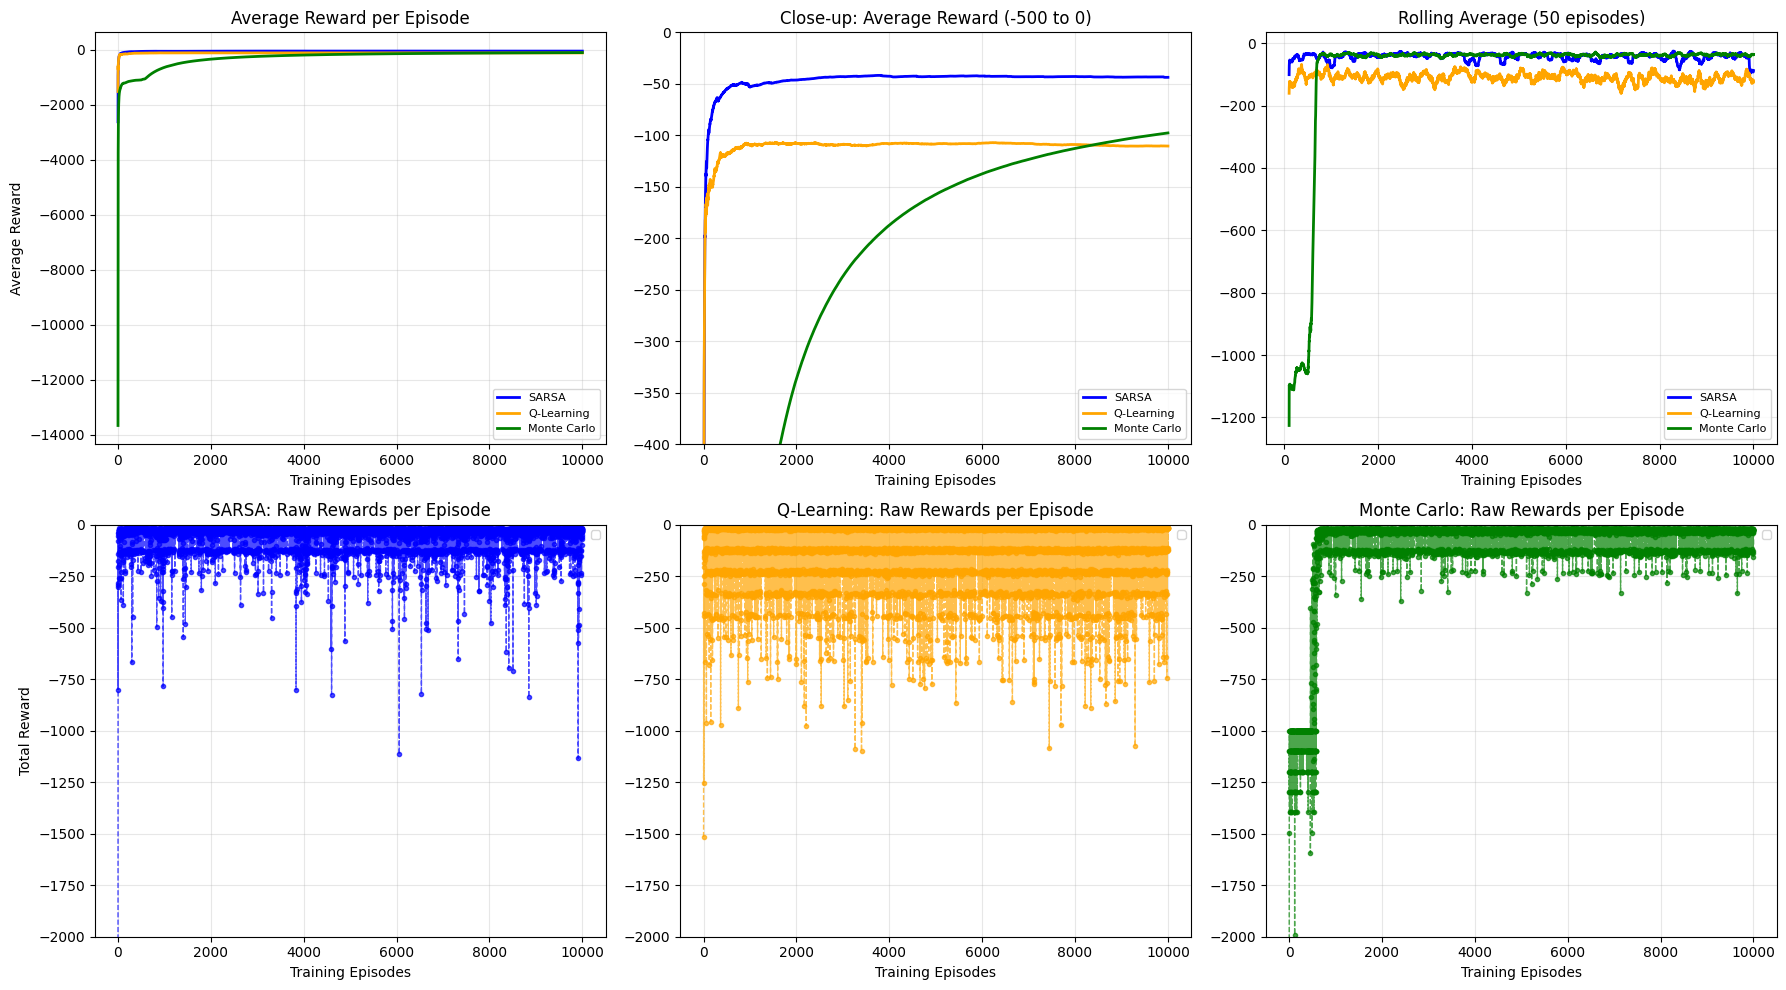
\includegraphics[width=0.8\textwidth]{Assignment1/Images/MC_Sarsa_Q2.png}
    \label{fig:yourlabel}
\end{figure}

\subsection{selection action function for algorithm in section 4.3 and 4.4}

\begin{lstlisting}
def select_action(state, Q, action_mask=None, epsilon=0.0):
    # If action_mask is not provided, consider all actions as valid
    valid_actions = np.where(action_mask == 1)[0] if action_mask is not None else np.arange(len(Q[state]))

    if np.random.rand() < epsilon:
        # Exploration: randomly choose among valid actions
        action_ = np.random.choice(valid_actions)
    else:
        # Exploitation: choose the best action among valid actions
        q_values_valid = Q[state][valid_actions]
        max_q = np.max(q_values_valid)
        
        # In case multiple actions have the same max Q-value, randomly choose among them
        best_actions = valid_actions[q_values_valid == max_q]
        action_ = np.random.choice(best_actions)

    return action_

\end{lstlisting}

\subsection{SARSA for Taxi Driver Environment without passing valid actions}

\begin{lstlisting}
alpha = 0.1
gamma = 0.99
epsilon = 0.1
num_episodes = 100000

Q = np.zeros((env.observation_space.n, env.action_space.n))

q_sum_of_rewards_per_episode = []

for episode in range(num_episodes):

    if (episode + 1) % 10000 == 0:
        print(f"Episode {episode + 1}/{num_episodes}")

    rewards = []

    # random state and i['action_mask] contains the actions that can be taken
    s, i = env.reset()

    while True:


        a = select_action(s, Q, None, epsilon)

        s_prime, r, is_done, is_terminated, i_prime = env.step(a)
        rewards.append(r)

        max_q_value = np.max(Q[s_prime])
        max_actions = np.where(Q[s_prime] == max_q_value)[0]
        chosen_action = np.random.choice(max_actions)
        max_q = Q[s_prime][chosen_action]  # This will be the same as max_q_value


        Q[s, a] += alpha * (r + gamma * max_q - Q[s, a])

        if is_done or is_terminated:
            break

        s = s_prime
        i = i_prime
    
    q_sum_of_rewards_per_episode.append(np.sum(rewards))
\end{lstlisting}

\subsection{Q-LEARNING for Taxi Driver Environment without passing valid actions}

\begin{lstlisting}
alpha = 0.1
gamma = 0.99
epsilon = 0.1
num_episodes = 100000

Q = np.zeros((env.observation_space.n, env.action_space.n))

q_sum_of_rewards_per_episode = []

for episode in range(num_episodes):

    if (episode + 1) % 10000 == 0:
        print(f"Episode {episode + 1}/{num_episodes}")

    rewards = []

    # random state and i['action_mask] contains the actions that can be taken
    s, i = env.reset()

    while True:


        a = select_action(s, Q, None, epsilon)

        s_prime, r, is_done, is_terminated, i_prime = env.step(a)
        rewards.append(r)

        max_q_value = np.max(Q[s_prime])
        max_actions = np.where(Q[s_prime] == max_q_value)[0]
        chosen_action = np.random.choice(max_actions)
        max_q = Q[s_prime][chosen_action]


        Q[s, a] += alpha * (r + gamma * max_q - Q[s, a])

        if is_done or is_terminated:
            break

        s = s_prime
        i = i_prime
    
    q_sum_of_rewards_per_episode.append(np.sum(rewards))
\end{lstlisting}

\pagebreak

\subsection{Graphs Performance with Different Epsilon Values}

\begin{figure}[h!]
    \centering
    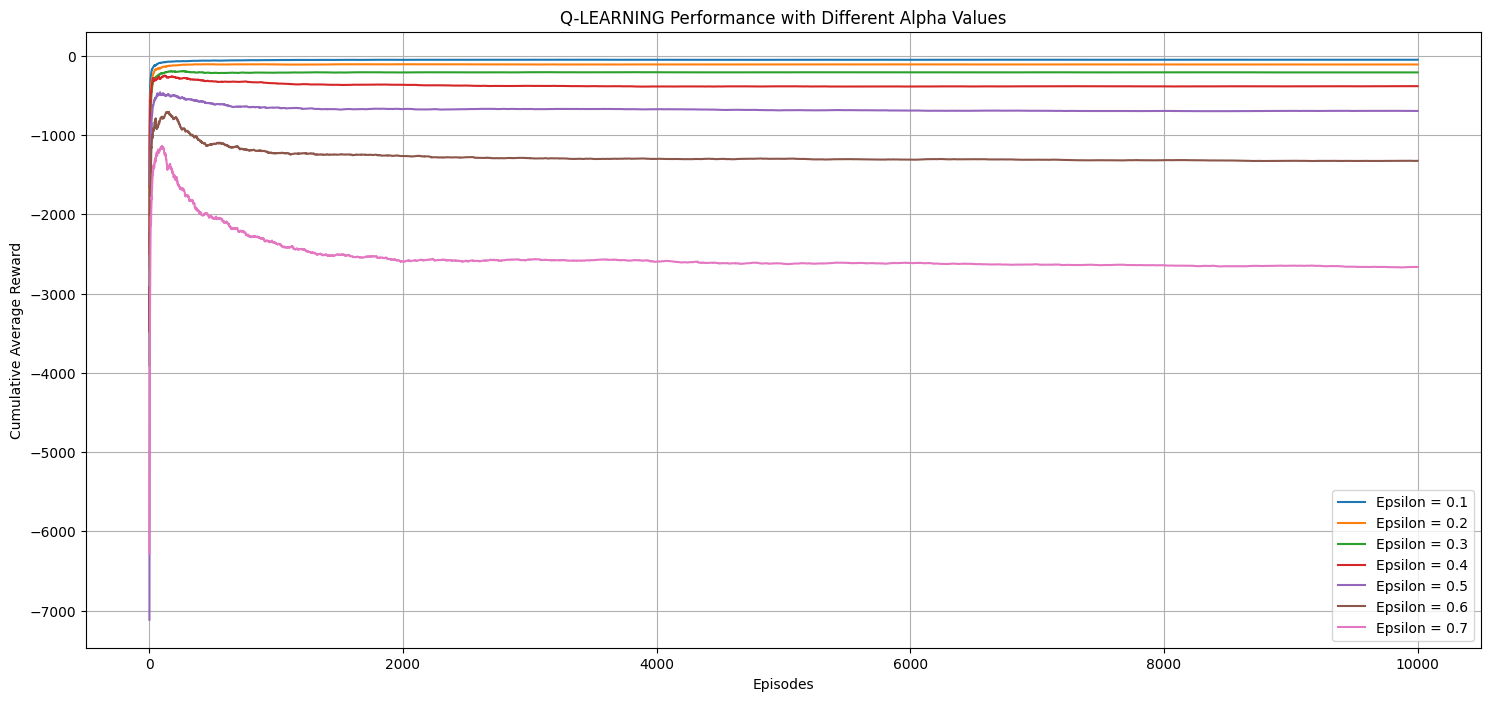
\includegraphics[width=0.77\textwidth]{Assignment1/Images/e_q.png}
    \caption{Performance with Different Epsilon Values Q-LEARNING}
    \label{fig:yourlabel}
\end{figure}

\begin{figure}[h!]
    \centering
    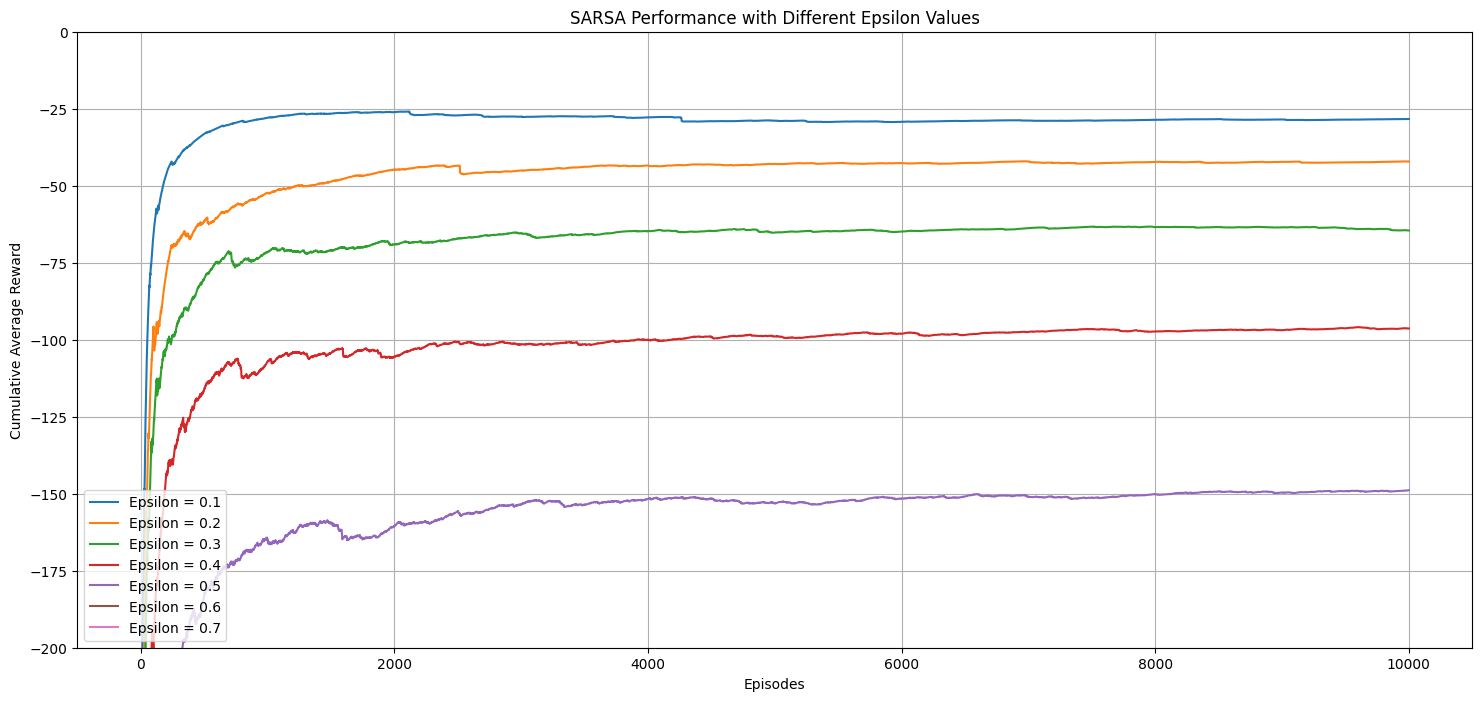
\includegraphics[width=0.77\textwidth]{Assignment1/Images/e_s.png}
    \caption{Performance with Different Epsilon Values SARSA}
    \label{fig:yourlabel}
\end{figure}

\begin{figure}[h!]
    \centering
    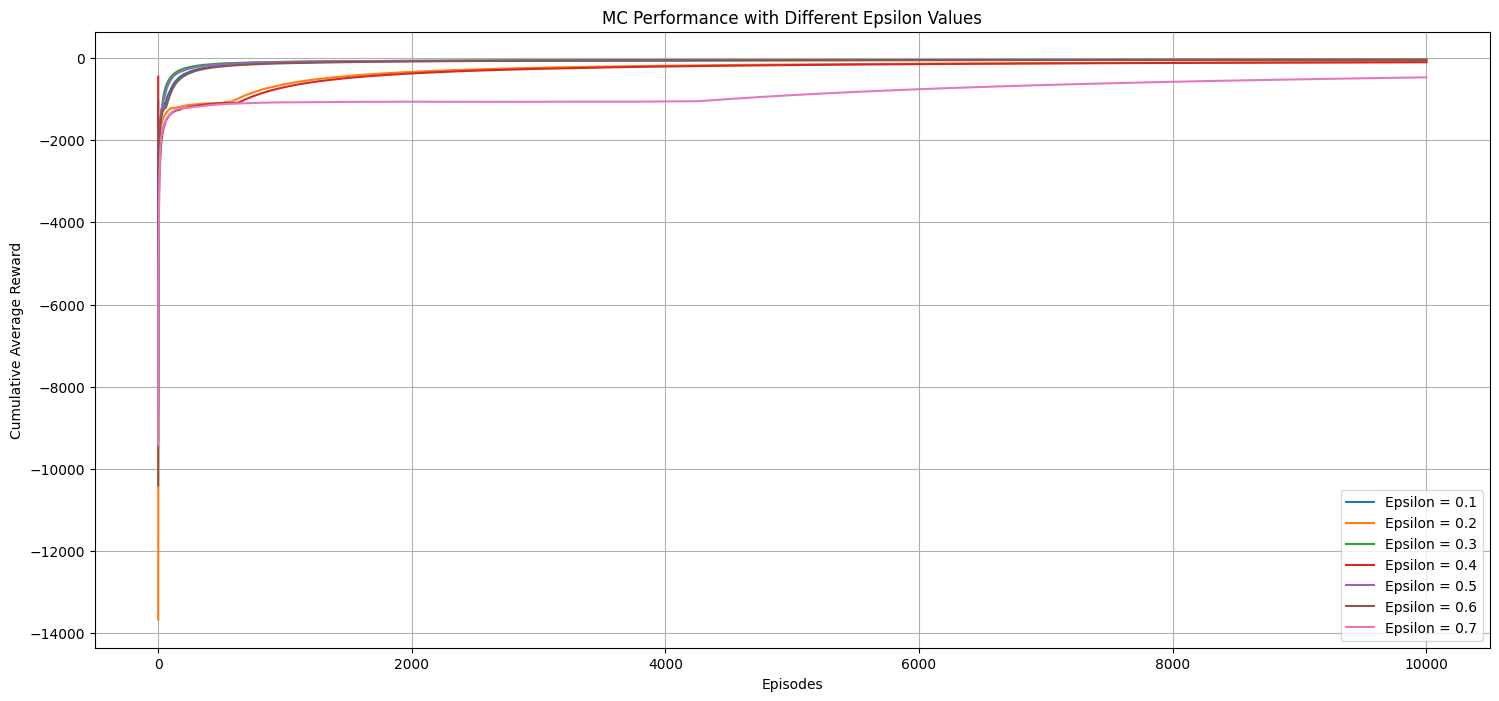
\includegraphics[width=0.77\textwidth]{Assignment1/Images/e_mc.png}
    \caption{Performance with Different Epsilon Values MC Control First-Visit}
    \label{fig:yourlabel}
\end{figure}

\pagebreak

\subsection{Algorithms taken from the book}

All the following algorithm pseudocodes have been taken from \textit{Reinforcement Learning: An Introduction} 2nd Edition by \textit{Richard S. Sutton \& Andrew G. Barto}

\begin{figure}[h!]
    \centering
    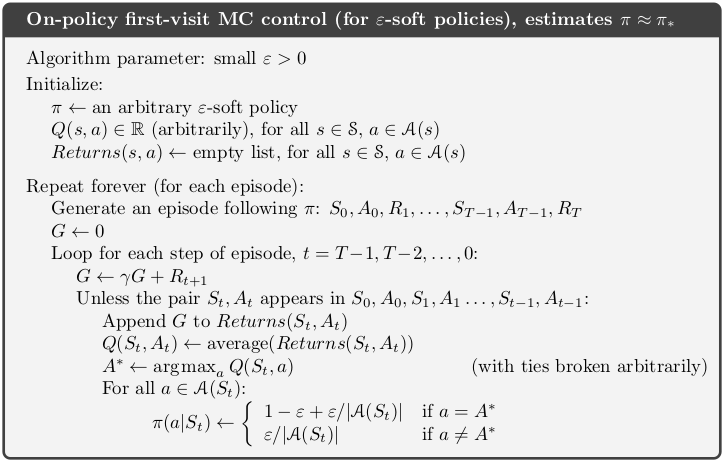
\includegraphics[width=0.77\textwidth]{Assignment1/Images/OnPolicy_MC_Ctrl.png}
\end{figure}

\begin{figure}[h!]
    \centering
    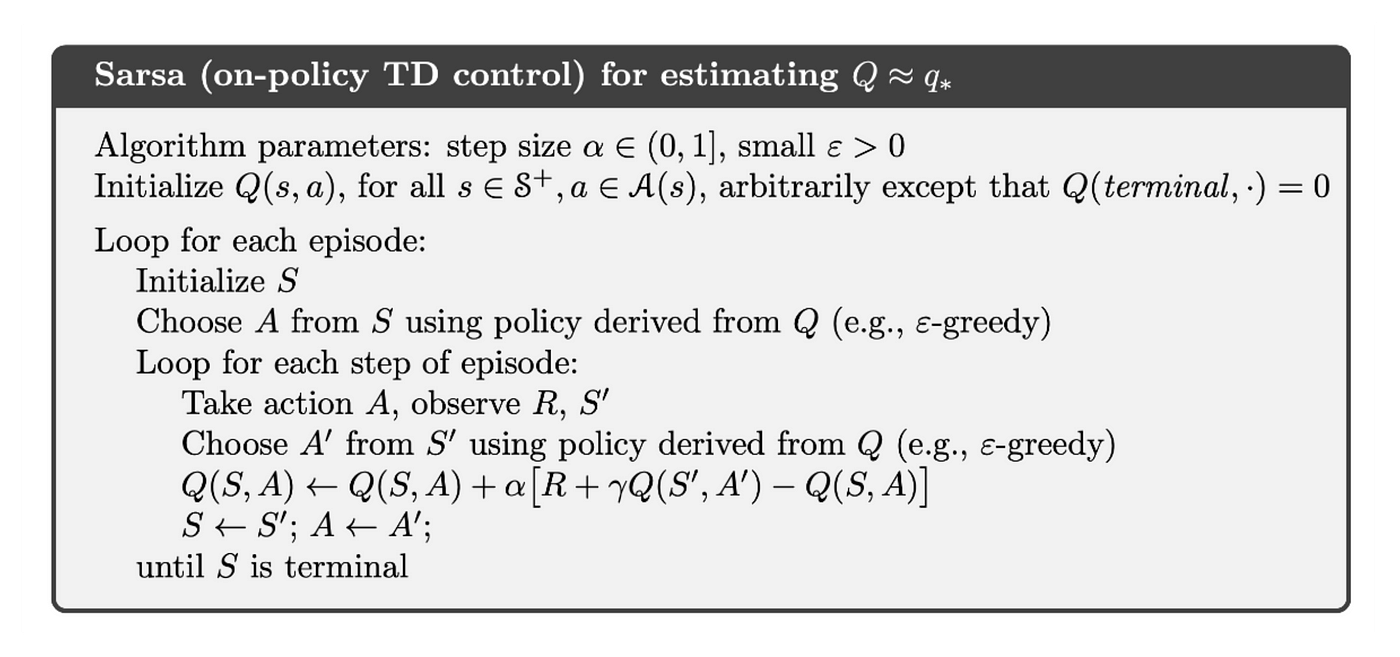
\includegraphics[width=0.8\textwidth]{Assignment1/Images/sarsa-barto.png}
\end{figure}

\begin{figure}[h!]
    \centering
    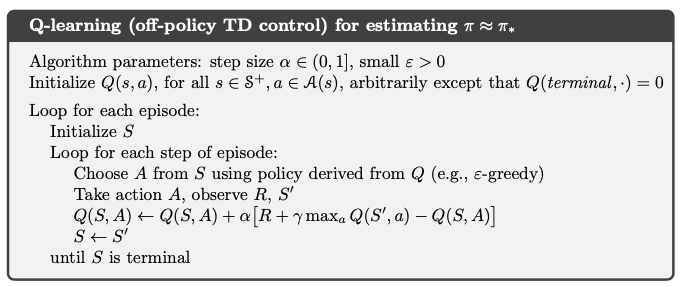
\includegraphics[width=0.78\textwidth]{Assignment1/Images/q-learning.png}
\end{figure}

\end{document}
